\begin{figure}[!ht]
    \centering
    \def\ncells{5}
    \begin{subfigure}[b]{0.3\columnwidth}
        \centering
        
\begin{tikzpicture}[scale=0.2]
            \draw[thin, opacity=0.2] (0, 0) grid (\ncells, \ncells);
        \end{tikzpicture}
        \caption{Square grid}
    \end{subfigure}
    %
    \begin{subfigure}[b]{0.3\columnwidth}
        \centering
        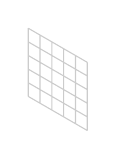
\begin{tikzpicture}[scale=0.15]
            \begin{scope}[thin, opacity=0.2, cm={1.0, -0.57735027, 0.0, 1.15470054, (0, 0)}]
                \draw[thin, opacity=0.2] (0, 0) grid (\ncells, \ncells);
            \end{scope}
        \end{tikzpicture}
        \vspace{-5pt}
        \caption{Skewed}
    \end{subfigure}
    %
    \begin{subfigure}[b]{0.3\columnwidth}
        \centering
        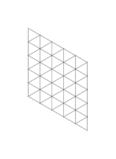
\begin{tikzpicture}[scale=0.15]
            \begin{scope}[thin, opacity=0.2, cm={1.0, -0.57735027, 0.0, 1.15470054, (0, 0)}]
                \foreach \x in {1, ..., \ncells}
                \foreach \y in {1, ..., \ncells}
                    \draw[thin, opacity=0.2] (\x - 1, \y - 1) -- (\x, \y - 1) -- (\x, \y) -- cycle;
                \draw (0, 0) -- (0, \ncells) -- (\ncells, \ncells);
            \end{scope}
        \end{tikzpicture}
        \vspace{-5pt}
        \caption{Triangulated\label{fig:surface-simplex-grid}}
    \end{subfigure}

    \vspace{-5pt}
    \caption{
        \cref{fig:surface-simplex-grid} shows the resulting simplex grid used for discretization of the surface position.
        \label{fig:surface-grid}
    }
\end{figure}